% +==============================================================+
% |  Projektopgave Dag 10-12                                     |
% |  Forfatter : aso                                             |
% |  Skole     : AAMS                                            |
% +==============================================================+

\documentclass[12pt, a4paper]{article}

% --- Kodning & sprog ----------------------------------------------------------
\usepackage[utf8]{inputenc}
\usepackage[T1]{fontenc}
\usepackage[danish]{babel}

% --- Layout -------------------------------------------------------------------
\usepackage{geometry}
\geometry{top=2.5cm, bottom=2.5cm, left=2.2cm, right=2.2cm, headheight=16pt}

% --- Typografi ----------------------------------------------------------------
\usepackage{lmodern}
\usepackage{microtype}
\usepackage{parskip}

% --- Grafik & farver ----------------------------------------------------------
\usepackage{graphicx}
\usepackage{xcolor}
\usepackage{tikz}
\usetikzlibrary{calc, arrows.meta, shapes.geometric, positioning, fit, backgrounds}

% --- Bokse & tabeller ---------------------------------------------------------
\usepackage[most]{tcolorbox}
\usepackage{enumitem}
\usepackage{booktabs}
\usepackage{array}
\usepackage{tabularx}
\usepackage{multirow}

% --- Header & footer ----------------------------------------------------------
\usepackage{fancyhdr}
\usepackage{titlesec}
\usepackage{fontawesome5}

% ==============================================================================
%  FARVEDEFINITIONER
% ==============================================================================
\definecolor{primaryblue}{HTML}{1A3A5C}
\definecolor{accentblue}{HTML}{2E86C1}
\definecolor{lightblue}{HTML}{D6EAF8}
\definecolor{darkgray}{HTML}{555555}
\definecolor{lightgray}{HTML}{F4F6F7}
\definecolor{successgreen}{HTML}{1E8449}
\definecolor{lightgreen}{HTML}{D5F5E3}
\definecolor{warnorange}{HTML}{E67E22}
\definecolor{lightyellow}{HTML}{FEF9E7}
\definecolor{siemensblue}{HTML}{009999}
\definecolor{passgreen}{HTML}{27AE60}

% --- Hyperlinks ---------------------------------------------------------------
\usepackage{hyperref}
\hypersetup{
  colorlinks = true,
  linkcolor  = primaryblue,
  urlcolor   = accentblue,
}

% ==============================================================================
%  TCOLORBOX STILE
% ==============================================================================
\tcbset{
  infobox/.style={
    enhanced, colback=lightblue, colframe=accentblue,
    coltitle=white, fonttitle=\bfseries, arc=3pt, boxrule=1pt,
    title style={fill=accentblue},
  },
  tipbox/.style={
    enhanced, colback=lightgreen, colframe=successgreen,
    coltitle=white, fonttitle=\bfseries, arc=3pt, boxrule=1pt,
    title style={fill=successgreen},
  },
  warnbox/.style={
    enhanced, colback=lightyellow, colframe=warnorange,
    coltitle=white, fonttitle=\bfseries, arc=3pt, boxrule=1pt,
    title style={fill=warnorange},
  },
  defbox/.style={
    enhanced, colback=lightgray, colframe=primaryblue,
    coltitle=white, fonttitle=\bfseries, arc=3pt, boxrule=1pt,
    title style={fill=primaryblue},
  },
}

% ==============================================================================
%  HEADER & FOOTER
% ==============================================================================
\pagestyle{fancy}
\fancyhf{}
\fancyhead[L]{\textcolor{darkgray}{\small\textit{Projektopgave Dag 10-12}}}
\fancyhead[R]{\textcolor{siemensblue}{\small\faIndustry}\;\textcolor{darkgray}{\small\textit{AAMS | aso}}}
\fancyhead[C]{}
\renewcommand{\headrulewidth}{1pt}
\renewcommand{\headrule}{{\color{siemensblue}\hrule height 1pt width\headwidth}}
\fancyfoot[C]{\textcolor{darkgray}{\small\thepage}}
\fancyfoot[R]{\textcolor{darkgray}{\small\today}}

% ==============================================================================
%  SEKTIONSFORMATERING
% ==============================================================================
\titleformat{\section}
  {\color{primaryblue}\Large\bfseries}
  {\color{siemensblue}\thesection\hspace{6pt}\textcolor{siemensblue}{|}\hspace{6pt}}
  {0pt}{}[{\color{siemensblue}\titlerule[1pt]}]

\titleformat{\subsection}
  {\color{primaryblue}\large\bfseries}
  {\color{accentblue}\thesubsection\hspace{6pt}}
  {0pt}{}

\titleformat{\subsubsection}
  {\color{primaryblue}\normalsize\bfseries}
  {\color{darkgray}\thesubsubsection\hspace{6pt}}
  {0pt}{}

\titlespacing{\section}{0pt}{18pt}{8pt}
\titlespacing{\subsection}{0pt}{12pt}{4pt}
\titlespacing{\subsubsection}{0pt}{8pt}{3pt}

% ==============================================================================
%  TIKZ STILE
% ==============================================================================
\tikzset{
  block/.style={
    rectangle, rounded corners=3pt, draw=primaryblue, thick,
    fill=lightblue, text width=3.2cm, align=center,
    minimum height=1.1cm, font=\small\bfseries\color{primaryblue}
  },
  sensor/.style={
    rectangle, rounded corners=3pt, draw=successgreen, thick,
    fill=lightgreen, text width=2.6cm, align=center,
    minimum height=0.9cm, font=\small\bfseries\color{successgreen!70!black}
  },
  actuator/.style={
    rectangle, rounded corners=3pt, draw=warnorange, thick,
    fill=lightyellow, text width=2.6cm, align=center,
    minimum height=0.9cm, font=\small\bfseries\color{warnorange!80!black}
  },
  software/.style={
    rectangle, rounded corners=3pt, draw=siemensblue, thick,
    fill=siemensblue!10, text width=3.2cm, align=center,
    minimum height=1.1cm, font=\small\bfseries\color{siemensblue!80!black}
  },
  myarrow/.style={-{Stealth[length=6pt]}, thick, color=darkgray},
  dbarrow/.style={-{Stealth[length=6pt]}, thick, color=siemensblue, dashed},
}

% ==============================================================================
%  DOKUMENT START
% ==============================================================================
\begin{document}
\pagenumbering{gobble}

% -----------------------------------------------------------------------------
%  FORSIDE
% -----------------------------------------------------------------------------
\begin{titlepage}
\thispagestyle{empty}


\begin{tikzpicture}[remember picture, overlay]
  \fill[primaryblue]
    (current page.north west) rectangle
    ([yshift=-4.5cm] current page.north east);
  \fill[siemensblue]
    ([yshift=-4.5cm] current page.north west) rectangle
    ([yshift=-5.0cm] current page.north east);
  \fill[accentblue]
    ([yshift=-5.0cm] current page.north west) rectangle
    ([yshift=-5.15cm] current page.north east);

  \node[anchor=east, xshift=-1.5cm, yshift=-2.3cm]
    at (current page.north east)
    {\textcolor{white!20!primaryblue}{\fontsize{90}{90}\selectfont\faProjectDiagram}};

  \node[anchor=north west, xshift=2cm, yshift=-0.7cm]
    at (current page.north west)
    {\textcolor{white!70!primaryblue}\large\bfseries AAMS --- Automationsteknolog};

  \node[anchor=north west, xshift=2cm, yshift=-1.3cm]
    at (current page.north west)
    {\textcolor{white!60!primaryblue}\normalsize Teknologi og Projektudvikling $\cdot$ 2.\ Semester};

  \node[anchor=north west, xshift=2cm, yshift=-2.2cm]
    at (current page.north west)
    {\textcolor{white}{\fontsize{22}{28}\selectfont\bfseries Projektopgave Dag 10-12}};

  \node[anchor=north west, xshift=2.1cm, yshift=-3.2cm]
    at (current page.north west)
    {\textcolor{white!80!siemensblue}\large\itshape
     PLC + Python + model/stand --- V-model, dokumentation og innovation};

  \node[anchor=north west, xshift=2.1cm, yshift=-3.85cm]
    at (current page.north west)
    {\textcolor{white!60!accentblue}\normalsize
     Kravspec. $\rightarrow$ Design $\rightarrow$ Kodning $\rightarrow$ Test $\rightarrow$ Demo};

  \fill[lightgray]
    ([yshift=3.5cm] current page.south west) rectangle
    ([yshift=2.0cm] current page.south east);
  \fill[accentblue]
    ([yshift=3.5cm] current page.south west) rectangle
    ([yshift=3.35cm] current page.south east);

  \node[anchor=west, xshift=2cm, yshift=2.8cm]
    at (current page.south west)
    {\textcolor{primaryblue}{\faUserCircle\quad\textbf{Forfatter:} aso
     \quad\textcolor{darkgray}{|}\quad
     \faCalendar\quad\textbf{Dato:} \today
     \quad\textcolor{darkgray}{|}\quad
     \faUniversity\quad\textbf{Skole:} AAMS}};
\end{tikzpicture}

\vspace*{5.5cm}

\begin{center}
\begin{tcolorbox}[
  enhanced, width=13cm, colback=lightgray, colframe=primaryblue,
  arc=5pt, boxrule=1.5pt,
  title={\faInfoCircle\quad Hvad går projektopgaven ud på?},
  coltitle=white, fonttitle=\bfseries, title style={fill=primaryblue},
]
I skal i \textbf{2-3-mandsgrupper} udvikle en prototype, hvor en
\textbf{PLC-løsning}, \textbf{Emulate3D eller standene i kælderen} og
\textbf{Python} indgår i samme løsning. I skal selv bruge \textbf{V-modellen}
som arbejdsmetode, og
dokumentationen må gerne ligne dokumentet
\textit{Eksempel: Vandstandsstyring med PLC og Python}.

\vspace{6pt}
\begin{itemize}[leftmargin=1.2em, itemsep=4pt]
  \item[\textcolor{siemensblue}{\faCheckCircle}]
    Brug Siemens PLC --- fysisk eller simuleret, det vælger I selv
  \item[\textcolor{siemensblue}{\faCheckCircle}]
    Brug Emulate3D, standene i kælderen eller en kombination som en del af jeres samlede løsning
  \item[\textcolor{siemensblue}{\faCheckCircle}]
    Brug Python til kommunikation, logik, logning, visualisering eller HMI
  \item[\textcolor{siemensblue}{\faCheckCircle}]
    Tilføj mindst ét nyt element ud over basisløsningen, f.eks. Rockwell + Siemens
  \item[\textcolor{siemensblue}{\faCheckCircle}]
    Afslut og demonstrér projektet på Dag 12
\end{itemize}
\end{tcolorbox}
\end{center}

\end{titlepage}
\clearpage
\pagenumbering{arabic}

% -----------------------------------------------------------------------------
%  INDHOLDSFORTEGNELSE
% -----------------------------------------------------------------------------
\newpage
\thispagestyle{fancy}
\tableofcontents
\newpage

% ==============================================================================
\section{Projektbeskrivelse}
% ==============================================================================

\subsection{Formål}

Projektet skal samle det vigtigste fra forløbet og vise, at I kan arbejde
systematisk fra idé til en demonstrerbar prototype. Fokus er ikke kun, at noget virker,
men at løsningen kan \textbf{forklares}, \textbf{dokumenteres} og
\textbf{testes}. Dette projekt er samtidig en \textbf{del af jeres aflevering}.

\begin{tcolorbox}[infobox, title={\faInfoCircle\quad Hvad skal projektet vise?}]
Projektet skal vise, at I kan:
\begin{itemize}[leftmargin=1.2em, itemsep=2pt]
  \item omsætte en idé til krav og design
  \item koble PLC, Python og enten Emulate3D, standene i kælderen eller en kombination sammen
  \item dokumentere i et format der må ligne \textit{Eksempel: Vandstandsstyring med PLC og Python}
  \item teste jeres løsning mod egne krav
  \item tilføje noget nyt, der giver reel ekstra funktionalitet
\end{itemize}
\end{tcolorbox}

\subsection{Grupper og rammer}

I arbejder i grupper af \textbf{2-3 personer}. Gruppen vælger selv, om jeres
Siemens PLC er \textbf{fysisk} eller \textbf{simuleret}. Det er også muligt at
arbejde med \textbf{Rockwell + Siemens} som en del af projektets nye element,
hvis det giver faglig mening. Det er et krav, at \textbf{Emulate3D},
\textbf{standene i kælderen} eller en kombination indgår i den samlede løsning.

Alle gruppemedlemmer skal fremgå med \textbf{navn}, \textbf{rolle i projektet}
og en kort beskrivelse af, hvad de hver især har \textbf{bidraget med}.

Derudover skal I anvende et \textbf{format der må ligne dokumentet}
\textit{Eksempel: Vandstandsstyring med PLC og Python}. Det betyder, at jeres
repo og dokumentation skal bygges op omkring samme faglige hoveddele:
systembeskrivelse, kravspecifikation, design, kodning, test og afsluttende
vurdering.
\clearpage
% ==============================================================================
\section{Systemramme}
% ==============================================================================

\subsection{Forventet systemopbygning}

Projektet må gerne have jeres eget scenarie, men det skal som minimum følge
denne overordnede struktur:

\begin{center}
\scalebox{0.9}{
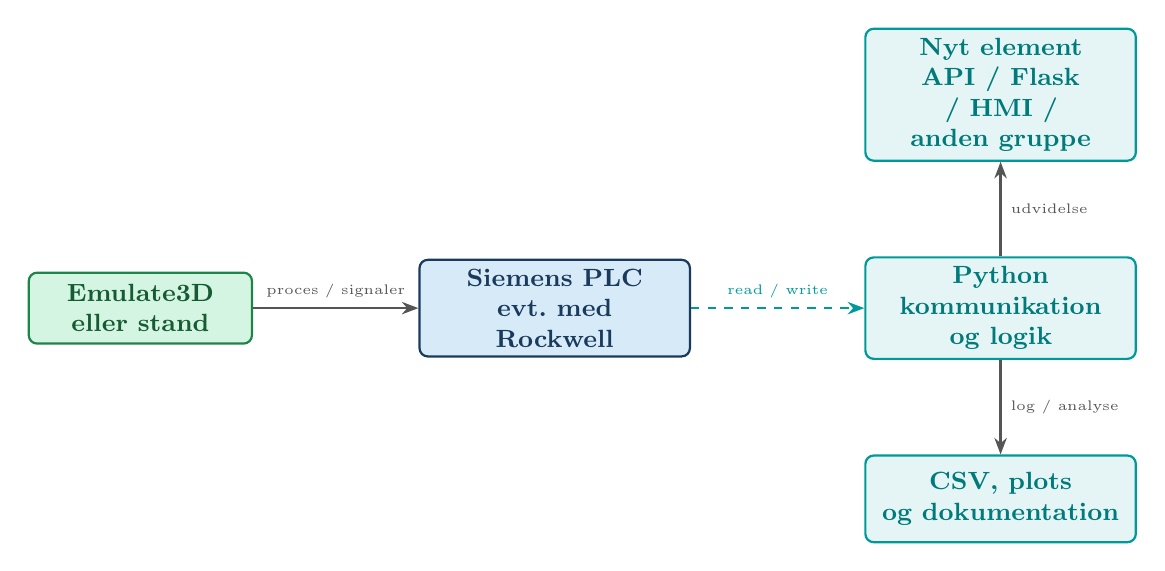
\begin{tikzpicture}[node distance=1.2cm and 2.3cm]

  \node[sensor] (emu) {Emulate3D\\eller stand};
  \node[block, right=2.1cm of emu] (plc) {Siemens PLC\\evt. med\\Rockwell};
  \node[software, right=2.2cm of plc] (py) {Python\\kommunikation\\og logik};
  \node[software, above=1.2cm of py, text width=3.2cm] (new)
    {Nyt element\\API / Flask / HMI /\\anden gruppe};
  \node[software, below=1.2cm of py, text width=3.2cm] (doc)
    {CSV, plots\\og dokumentation};

  \draw[myarrow] (emu.east) -- node[above, font=\tiny\color{darkgray}]
    {proces / signaler} (plc.west);
  \draw[dbarrow] (plc.east) -- node[above, font=\tiny\color{siemensblue}]
    {read / write} (py.west);
  \draw[myarrow] (py.north) -- node[right, font=\tiny\color{darkgray}]
    {udvidelse} (new.south);
  \draw[myarrow] (py.south) -- node[right, font=\tiny\color{darkgray}]
    {log / analyse} (doc.north);

\end{tikzpicture}
}
\end{center}

\begin{tcolorbox}[tipbox, title={\faCheckSquare\quad Vigtigt}] 
Python må gerne bruges til flere roller samtidigt: kommunikation, HMI,
visualisering, webserver, dataudveksling, alarmer eller rapportering. Det er
ikke nok kun at læse lidt data og printe dem i terminalen.
\end{tcolorbox}
\clearpage
% ==============================================================================
\section{Opgavens rammer}
% ==============================================================================

\subsection{Det skal indgå i projektet}

\begin{center}
\begin{tabularx}{\textwidth}{>{\raggedright\arraybackslash}p{0.31\textwidth} X}
\toprule
\textbf{Fast del} & \textbf{Det betyder i praksis} \\
\midrule
Gruppe på 2-3 & I afleverer og demonstrerer som én samlet gruppe, og alle skal skrive navn, rolle og eget bidrag ind i materialet. \\[6pt]
PLC & PLC'en må være fysisk eller simuleret, og Siemens skal være en reel del af den løsning I viser frem. Rockwell må gerne kobles på som et nyt element. \\[6pt]
Model/stand & Emulate3D, standene i kælderen eller en kombination skal indgå som model, proces eller fysisk visning af anlægget. \\[6pt]
Python & Python skal give reel værdi i systemet, f.eks. gennem kommunikation, logik, logning, visualisering eller HMI. \\[6pt]
Nyt element & Løsningen skal udvides med mindst ét ekstra element, som kan forklares og demonstreres. \\[6pt]
Afleveringsformat & I skal aflevere en rapport som PDF, en video og hele projektet enten som zip-fil eller som GitHub-repo. Valget mellem zip og repo er jeres. \\[6pt]
Afslutning på Dag 12 & Projektet skal være samlet nok til demonstration, testet så langt som muligt og klar til aflevering og demo på sidste dag. \\
\bottomrule
\end{tabularx}
\end{center}

\subsection{Det vælger I selv}

\begin{tcolorbox}[infobox, title={\faInfoCircle\quad Jeres egne valg}]
I vælger selv scenarie, proces, signaler og systemopbygning, så længe jeres
løsning giver faglig mening. I bestemmer også selv, om PLC'en er fysisk eller
simuleret, om I vil bruge Emulate3D, standene i kælderen eller begge dele, og
hvordan Python skal give værdi i jeres samlede løsning.
\end{tcolorbox}

% ==============================================================================
\section{Dokumentation og arbejdsform}
% ==============================================================================

\subsection{Sådan skal I arbejde}

I skal selv bruge V-modellen som arbejdsmetode, så der er tydelig sammenhæng
mellem idé, krav, design, implementering og test. Dokumentationen må gerne
ligne dokumentet \textit{Eksempel: Vandstandsstyring med PLC og Python}, men
det er jer selv, der skal definere indholdet ud fra jeres eget system.

\begin{tcolorbox}[defbox, title={\faCheckSquare\quad Det skal jeres materiale vise}]
Jeres repo og dokumentation skal som minimum indeholde:
\begin{itemize}[leftmargin=1.2em, itemsep=2pt]
  \item en kort systembeskrivelse
  \item en kravspecifikation med acceptkriterier
  \item et blokdiagram og en relevant designbeskrivelse
  \item et flowchart eller en state machine for Python-delen
  \item en forklaring af samspillet mellem PLC, Python og jeres valgte model-, stand- eller kombinationsløsning
  \item testdokumentation med tydelige resultater
  \item en kort afsluttende vurdering eller konklusion
  \item en forklaring af jeres valg og relevante fravalg gennem hele V-modellen
\end{itemize}
\end{tcolorbox}

\begin{tcolorbox}[warnbox, title={\faExclamationTriangle\quad Det her er vigtigt}]
Det er ikke nok at aflevere kodefiler alene. Gruppen skal vise, hvordan
løsningen hænger sammen fra krav til test. Dokumentationen skal passe til det
system I faktisk har bygget --- ikke til en idé I havde tidligere på dagen.
\end{tcolorbox}

\subsection{Det I selv skal udarbejde}

\begin{tcolorbox}[tipbox, title={\faCheckSquare\quad Jeres eget projektmateriale}]
I skal selv udarbejde det konkrete indhold til jeres løsning. Det betyder, at
I selv formulerer og begrunder:
\begin{itemize}[leftmargin=1.2em, itemsep=2pt]
  \item jeres systembeskrivelse og scenarie
  \item jeres krav og acceptkriterier
  \item jeres blokdiagram og logikbeskrivelse
  \item jeres flowchart eller state machine
  \item jeres testoversigt og vurdering af resultaterne
\end{itemize}
\end{tcolorbox}

% ==============================================================================
\section{Noget nyt: Obligatorisk innovation}
% ==============================================================================

\subsection{Mindst ét nyt element}

Projektet skal indeholde mindst ét nyt element, som går ud over basisløsningen.
Det må gerne være simpelt, men det skal være \textbf{meningsfuldt} og kunne
\textbf{demonstreres tydeligt}.

\begin{center}
\begin{tabularx}{\textwidth}{lXX}
\toprule
\textbf{Valg} & \textbf{Hvad det kan være} & \textbf{Hvordan det kan demonstreres} \\
\midrule
Ekstern kommunikation & Dataudveksling med en anden gruppe, f.eks. status, alarm eller produktionstal & Begge grupper kan sende eller modtage en relevant værdi eller besked \\[6pt]

API & Kald til et API eller eksponering af egne data via et endpoint & Python læser eller sender data gennem en defineret API-forbindelse \\[6pt]

Flask-server & En lille lokal webserver med status, alarmer eller kommandoer & Der vises en browserbaseret side eller et endpoint som del af løsningen \\[6pt]

Python-HMI & Lokalt HMI i Python, f.eks. Tkinter eller tilsvarende & Operatøren kan se status og evt. sende kommandoer via et interface \\[6pt]

Andet & En anden idé godkendt af underviseren & Gruppen kan forklare værdien og vise at funktionen virker \\
\bottomrule
\end{tabularx}
\end{center}

\vspace{0.2cm}
\noindent\textbf{Bemærk:} Et muligt nyt element kan også være at koble
\textbf{Rockwell + Siemens} sammen, hvis gruppen kan begrunde valget og vise,
hvordan det giver faglig værdi i løsningen.

\begin{tcolorbox}[tipbox, title={\faStar\quad God tommelfingerregel}]
Det nye element skal ikke bare være pynt. Det skal give jeres løsning en ekstra
funktion, som gør systemet mere realistisk, mere brugbart eller mere interessant
at demonstrere.
\end{tcolorbox}

% ==============================================================================
\section{Arbejde fordelt på dagene}
% ==============================================================================

Her er fokus på, hvad I skal arbejde med gennem forløbet. Det er ikke tænkt som
separate afleveringer per dag, men som en tydelig ramme for projektarbejdet.

\begin{tabularx}{\textwidth}{lXX}
\toprule
\textbf{Dag} & \textbf{Fokus} & \textbf{Det I skal arbejde med} \\
\midrule
Dag 10 & Krav, design og plan & Gruppedannelse, projektidé, kravspecifikation, acceptkriterier, blokdiagram, flowchart eller state machine samt valg af nyt element \\[6pt]

Dag 11 & Implementering og integration & PLC-kommunikation i Python, kobling til Emulate3D, stand eller tilsvarende løsning, logning til fil og første version af det nye element \\[6pt]

Dag 12 & Test, dokumentation og afslutning & Samlet og demonstrerbar løsning, test mod egne krav, endelig dokumentation, demo og aflevering \\
\bottomrule
\end{tabularx}
\clearpage
% ==============================================================================
\section{Aflevering og vurdering}
% ==============================================================================

\subsection{Det der skal afleveres}

Dette projekt er en del af jeres aflevering. I skal aflevere:

\begin{itemize}[leftmargin=1.2em, itemsep=2pt]
  \item en rapport som \textbf{PDF}
  \item en \textbf{video}, hvor projektet og løsningen vises eller forklares
  \item hele projektet enten som \textbf{zip-fil} eller som \textbf{GitHub-repo} --- valget er jeres
\end{itemize}

Rapporten og det samlede projektmateriale skal som minimum indeholde:

\begin{itemize}[leftmargin=1.2em, itemsep=2pt]
  \item forside eller afsnit med alle gruppemedlemmers navne
  \item kort beskrivelse af hver persons rolle i projektet
  \item kort beskrivelse af hvad hver person har bidraget med
  \item kort projektbeskrivelse
  \item kravspecifikation med acceptkriterier
  \item blokdiagram
  \item flowchart eller state machine
  \item Python-kode
  \item relevant beskrivelse af PLC-tags, signaler eller dataudveksling
  \item screenshots eller billeder fra Emulate3D, stand, HMI eller tests
  \item logfil eller CSV-eksempel
  \item testoversigt med pass/fail
  \item beskrivelse af det nye element
  \item kort forklaring af valg og relevante fravalg gennem V-modellen
\end{itemize}

\subsection{Hvad der lægges vægt på}

\begin{tcolorbox}[defbox, title={\faTasks\quad Vurdering}] 
Der lægges vægt på:
\begin{itemize}[leftmargin=1.2em, itemsep=4pt]
  \item at PLC, Python og den valgte model-, stand- eller kombinationsløsning spiller sammen
  \item at der er tydelig sammenhæng mellem krav, design, implementering og test
  \item at krav og test kan spores til hinanden
  \item at Python-løsningen giver reel ekstra funktionalitet
  \item at det nye element virker og giver mening
  \item at det er tydeligt, hvem der har haft hvilke roller og bidrag i projektet
  \item at gruppen kan forklare alle trin i V-modellen samt deres valg og relevante fravalg fra start til slut
  \item at gruppen kan demonstrere resultatet tydeligt på Dag 12
\end{itemize}
\end{tcolorbox}

\begin{tcolorbox}[warnbox, title={\faFlagCheckered\quad Afslutning}]
Projektet afsluttes på \textbf{Dag 12}. Det er ikke nok at have noget der
kun delvist hænger sammen. Løsningen behøver ikke være 100\% færdig, men den skal være
så langt, at gruppen kan demonstrere den meningsfuldt og vise, at den er
dokumenteret, testet og forstået. Gruppen skal desuden kunne forklare hele
forløbet gennem V-modellen, herunder deres valg og relevante fravalg fra start
til slut.
\end{tcolorbox}

\end{document}